
\documentclass{beamer}
%https://en.wikibooks.org/wiki/LaTeX/Macros
\usepackage{tikz}
%vectors, matrices, complex numbers,  trigonometrie, big O notation, grafentheorie, vertaling van probleem in algoritme,
\useoutertheme{infolines}
\newcommand{\drawgridaxes}{
\draw[step=1cm,gray,very thin] (-3,-3) grid (3,3);
\draw[thick,->] (0,0) -- (3,0) node[anchor=north west] {x};
\draw[thick,->] (0,0) -- (0,3) node[anchor=south east] {y};
\draw[thick,->] (0,0) -- (-3,0);
\draw[thick,->] (0,0) -- (0,-3);
}

\newcommand{\drawtdvec}[2]{
\begin{tikzpicture}[scale=0.70]
\drawgridaxes
\draw[red, thick, ->] (0,0) -- (#1,#2);
\end{tikzpicture}
}

\newcommand{\drawbasicvec}{
		\begin{equation*} \vec{V} = \begin{bmatrix} 1 \\ 2 \end{bmatrix} \end{equation*}

        \drawtdvec{1}{2}
}

\newcommand{\tcframe}[3] {
	\frame {
		\frametitle{#1}
\begin{columns}
\begin{column}{0.5\textwidth}
		#2
\end{column}

\begin{column}{0.5\textwidth}
		#3
\end{column}
\end{columns}
}
}

\definecolor{darkgreen}{RGB}{0,150,0}


\title{Some math}
\subtitle{Random things you might encounter in the core or afterwards}

\begin{document}
	\frame {
		\titlepage
	}
	
	\tcframe{Vector, representation}
	{\drawbasicvec}
	{\begin{equation*} \textbf{U} = \begin{bmatrix} 0.2 \\ 0.5 \\ 0.7 \\ 0.2 \\ 0.2 \\ 0.2 \end{bmatrix} \end{equation*} \drawtdvec{1.1}{1.7}}
	
	\tcframe{Scaling a vector}
	{\drawbasicvec}
	{\begin{equation*} 1.5 * \vec{V} = \begin{bmatrix} 1.5 \\ 3  \end{bmatrix} \end{equation*}
		\drawtdvec{1.5}{3}}
		
			\tcframe{Scaling with negative number}
	{\drawbasicvec}
	{\begin{equation*} -1.5 * \vec{V} = \begin{bmatrix} -1.5 \\ -3  \end{bmatrix} \end{equation*}
		\drawtdvec{-1.5}{-3}}
	
	\frame {
		\frametitle{Scaling all happens on the same line}
		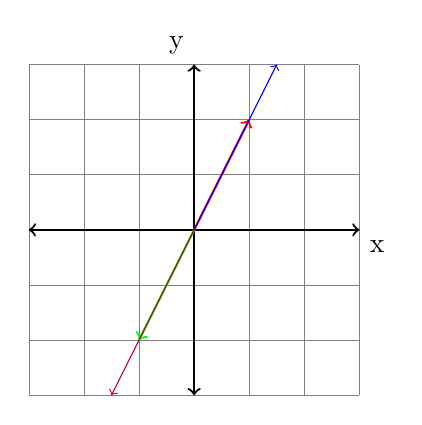
\begin{tikzpicture}[scale=0.70]
        \drawgridaxes
        \draw[red, thick, ->] (0,0) -- (1,2);
        \draw[green, thick, ->] (0,0) -- (-1,-2);
        \draw[blue, ->] (0,0) -- (1.5,3);
        \draw[purple, ->] (0,0) -- (-1.5,-3);
        \end{tikzpicture}
	}
	
	\frame {
		\frametitle{Adding vectors, or splitting up in components}
		\begin{equation*} \begin{bmatrix} 2 \\ 0 \end{bmatrix} + \begin{bmatrix} 0 \\ 1 \end{bmatrix} = \begin{bmatrix} 2 \\ 1 \end{bmatrix}\end{equation*}
		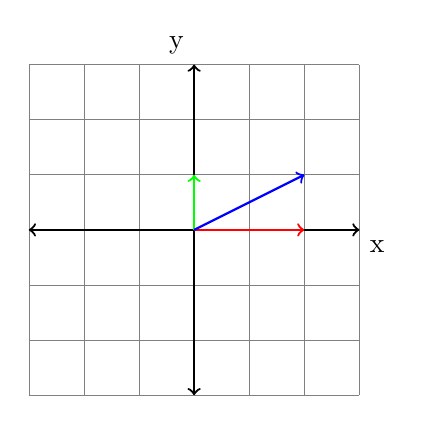
\begin{tikzpicture}[scale=0.70]
        \drawgridaxes
        \draw[red, thick, ->] (0,0) -- (2,0);
        \draw[green, thick, ->] (0,0) -- (0,1);
        \draw[blue, thick, ->] (0,0) -- (2,1);
        \end{tikzpicture}
	}
	
	\frame {
		\frametitle{Subtracting vectors}
		\begin{equation*} \begin{bmatrix} 2 \\ 1 \end{bmatrix} - \begin{bmatrix} 2 \\ 0 \end{bmatrix} = \begin{bmatrix} 0 \\ 1 \end{bmatrix}\end{equation*}
		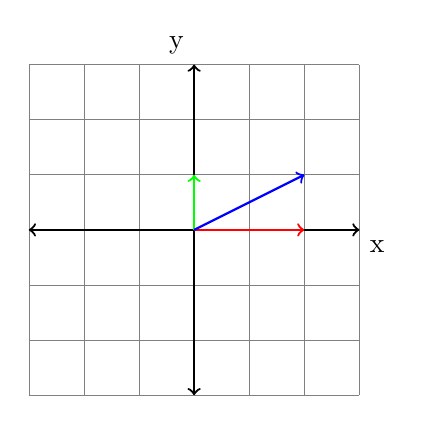
\begin{tikzpicture}[scale=0.70]
        \drawgridaxes
        \draw[red, thick, ->] (0,0) -- (2,0);
        \draw[green, thick, ->] (0,0) -- (0,1);
        \draw[blue, thick, ->] (0,0) -- (2,1);
        \end{tikzpicture}
	}
	
	\frame {
		\frametitle{Matrix, representation}
		\begin{equation*} \textbf{M} = \begin{bmatrix} 0.2 & 0.3 \\ 0.5 & 0.6 \end{bmatrix} \end{equation*}
		\begin{equation*} \textbf{N} = \begin{bmatrix} 0.2 & 0.3 & 5 & 6 \\ 0.5 & 0.6 & 7 & 8 \end{bmatrix} \end{equation*}
	}
	\frame {
		\frametitle{Multiplying matrix with a vector}
		\begin{equation*} \textbf{M} = \begin{bmatrix} a & b \\ c & d \end{bmatrix} * \begin{bmatrix} v1 \\ v2 \end{bmatrix} = \begin{bmatrix} a * v1 + b * v2 \\ c * v1 + d * v2 \end{bmatrix}\end{equation*}
		\begin{equation*} \textbf{M} = \begin{bmatrix} 1 & 2 \\ 3 & 4 \end{bmatrix} * \begin{bmatrix} 5 \\ 6 \end{bmatrix} = \begin{bmatrix} 1 * 5 + 2 * 6 \\ 3 * 5 + 4 * 6 \end{bmatrix} = \begin{bmatrix} 17 \\ 39 \end{bmatrix}\end{equation*}
	}
	\frame {
		\frametitle{Identity matrix}
		\begin{equation*} \textbf{M} = \begin{bmatrix} 1 & 0 \\ 0 & 1 \end{bmatrix} * \begin{bmatrix} 5 \\ 6 \end{bmatrix} = \begin{bmatrix} 1 * 5 + 0 * 6 \\ 0 * 5 + 1 * 6 \end{bmatrix} = \begin{bmatrix} 5 \\ 6 \end{bmatrix}\end{equation*}
	}
	\frame {
		\frametitle{90 degrees rotation matrix}
		\begin{equation*} \textbf{M} = \begin{bmatrix} 0 & -1 \\ 1 & 0 \end{bmatrix} * \begin{bmatrix} 1 \\ 2 \end{bmatrix} = \begin{bmatrix} 0 * 1 + -1 * 2 \\ 1 * 1 + 0 * 2 \end{bmatrix} = \begin{bmatrix} -2 \\ 1 \end{bmatrix}\end{equation*}
		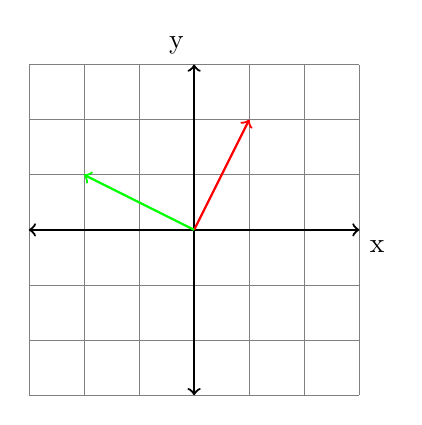
\begin{tikzpicture}[scale=0.70]
        \drawgridaxes
        \draw[red, thick, ->] (0,0) -- (1,2);
        \draw[green, thick, ->] (0,0) -- (-2,1);
        \end{tikzpicture}
	}
	\frame {
		\frametitle{Sin and Cos, rotation from x-axis}
		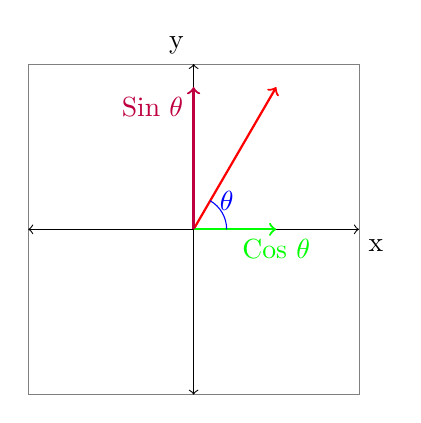
\begin{tikzpicture}[scale=2.10]
		\draw[step=1cm,gray,very thin] (-1,-1) grid (1,1);
        \draw[thin,->] (0,0) -- (1,0) node[anchor=north west] {x};
        \draw[thin,->] (0,0) -- (0,1) node[anchor=south east] {y};
        \draw[thin,->] (0,0) -- (-1,0);
        \draw[thin,->] (0,0) -- (0,-1);
        \draw[red, thick, ->] (0,0) -- (0.5,0.86);
        \draw[green, thick, ->] (0,0) -- (0.5,0) node[below] {Cos $\theta$};
        \draw[purple, thick, ->] (0,0) -- (0,0.86) node[anchor=north east] {Sin $\theta$};
        \draw[blue] (0.2,0) arc (0:60:0.2cm) node[right] {$\theta$};
        \end{tikzpicture}
	}
	
	\frame {
		\frametitle{Sin and Cos, rotation from y-axis}
		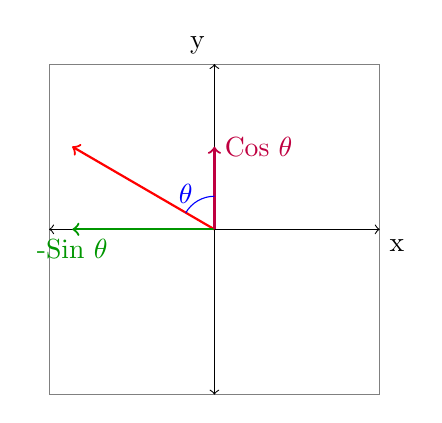
\begin{tikzpicture}[scale=2.10]
		\draw[step=1cm,gray,very thin] (-1,-1) grid (1,1);
        \draw[thin,->] (0,0) -- (1,0) node[anchor=north west] {x};
        \draw[thin,->] (0,0) -- (0,1) node[anchor=south east] {y};
        \draw[thin,->] (0,0) -- (-1,0);
        \draw[thin,->] (0,0) -- (0,-1);
        \draw[red, thick, ->] (0,0) -- (-0.86,0.5);
        \draw[darkgreen, thick, ->] (0,0) -- (-0.86,0) node[below] {-Sin $\theta$};
        \draw[purple, thick, ->] (0,0) -- (0,0.5) node[right] {Cos $\theta$};
        \draw[blue] (0,0.2) arc (90:150:0.2cm) node[above] {$\theta$};
        \end{tikzpicture}
	}
	
	\frame {
		\frametitle{Rotation matrix}
		\begin{equation*} \textbf{M} = \begin{bmatrix} \cos(\theta) & -\sin(\theta) \\ \sin(\theta) & \cos( \theta) \end{bmatrix} * \begin{bmatrix} x \\ y \end{bmatrix} = \begin{bmatrix} \cos(\theta) * x - \sin(\theta) * y \\ \sin(\theta)  * x + \cos(\theta) * y \end{bmatrix}
		\end{equation*}
	}
	
	\frame {
		\frametitle{Complex numbers}
		\begin{equation*} c = a + bi
		\end{equation*}
	    \begin{equation*} i^2 = -1
		\end{equation*}
	}
	
	\frame {
		\frametitle{Complex numbers, addition}
		\begin{equation*} (a_1 + b_1i) + a_2 = (a_1 + a_2) + b_1i 
		\end{equation*}
		\begin{equation*} (a_1 + b_1i) + b_2i = a_1 + (b_1 + b_2)i 
		\end{equation*}
		\begin{equation*} (a_1 + b_1i) + (a_2 + b_2i) = (a_1 + a_2) + (b_1 + b_2)i 
		\end{equation*}
	}
	
	\frame {
		\frametitle{Complex numbers, multiplication}
		\begin{equation*} (a_1 + b_1i) * (a_2 + b_2i) = (a_1 * a_2) + (a_1 * b_2i) + (b_1i * a_2) + (b_1i * b_2i) 
		\end{equation*}
		\begin{equation*}
		= (a_1 * a_2) + (a_1 * b_2 + b_1 * a_2)i + (b_1 * b_2)i^2 
		\end{equation*}
			\begin{equation*}
		=  a_1 * a_2 + (a_1 * b_2 + b_1 * a_2)i - (b_1 * b_2)
			\end{equation*}
		\begin{equation*}
		= (a_1 * a_2 - b_1 * b_2) + (a_1 * b_2 + b_1 * a_2)i
		\end{equation*}
	}
	
	\frame {
		\frametitle{Complex numbers, vector and matrix}
		\begin{equation*} (a_1 + b_1i) * (a_2 + b_2i)
		\end{equation*}
		\begin{equation*}
		= (a_1 * a_2 - b_1 * b_2) + (a_1 * b_2 + b_1 * a_2)i
		\end{equation*}
		\begin{equation*}
		= \begin{bmatrix} a_1 & -b_1 \\ b_1 & a_1 \end{bmatrix} * \begin{bmatrix} a_2 \\ b_2 \end{bmatrix}
		\end{equation*}
	}
	
	\frame {
		\frametitle{Complex numbers, rotation}
		\begin{equation*} (\cos(\theta) + i*\sin(\theta)) * (a_2 + b_2i)
		\end{equation*}
		\begin{equation*}
		= \begin{bmatrix} \cos(\theta) & -\sin(\theta) \\ \sin(\theta) & \cos(\theta) \end{bmatrix} * \begin{bmatrix} a_2 \\ b_2 \end{bmatrix}
		\end{equation*}
	}
	
	\frame {
		\frametitle{Complex numbers, rotation picture}
		\begin{equation*} (\cos(\theta) + i*\sin(\theta)) * (a_2 + b_2i)
		\end{equation*}
		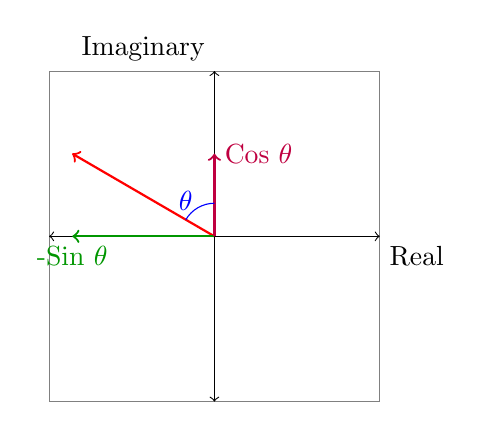
\begin{tikzpicture}[scale=2.10]
		\draw[step=1cm,gray,very thin] (-1,-1) grid (1,1);
        \draw[thin,->] (0,0) -- (1,0) node[anchor=north west] {Real};
        \draw[thin,->] (0,0) -- (0,1) node[anchor=south east] {Imaginary};
        \draw[thin,->] (0,0) -- (-1,0);
        \draw[thin,->] (0,0) -- (0,-1);
        \draw[red, thick, ->] (0,0) -- (-0.86,0.5);
        \draw[darkgreen, thick, ->] (0,0) -- (-0.86,0) node[below] {-Sin $\theta$};
        \draw[purple, thick, ->] (0,0) -- (0,0.5) node[right] {Cos $\theta$};
        \draw[blue] (0,0.2) arc (90:150:0.2cm) node[above] {$\theta$};
        \end{tikzpicture}
	}
	
	%https://en.wikipedia.org/wiki/Complex_number#Matrix_representation_of_complex_numbers
	
	\frame {
		\begin{equation*} a*x^2 + b*x + c = 0
		\end{equation*}
		\frametitle{ABC formula}
		\[\frac{-b \pm \sqrt{b^2 - 4 a c}}{2a}\]
		\begin{equation*} b^2 - 4 a c >= 0
		\end{equation*}
	}
	
	\frame {
		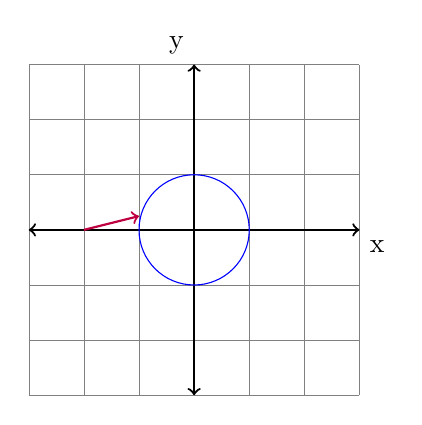
\begin{tikzpicture}[scale=0.7]
        \drawgridaxes
        \draw[purple, thick, ->] (-2,0) -- (-1,0.25);
        \draw[blue] (0,0) circle (1cm);
        \end{tikzpicture}
	}
	
	\frame {
		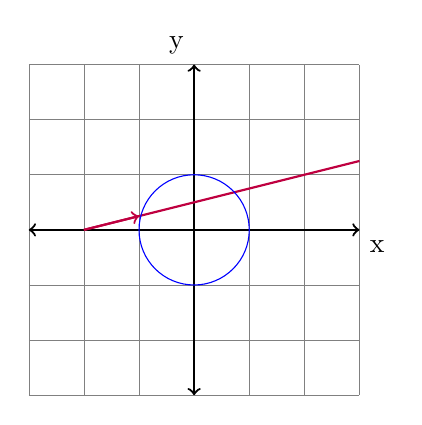
\begin{tikzpicture}[scale=0.7]
        \drawgridaxes
        \draw[purple, thick, ->] (-2,0) -- (-1,0.25);
        \draw[purple, thick] (-2,0) -- (3,1.25);
        \draw[blue] (0,0) circle (1cm);
        \end{tikzpicture}
	}
	
	\frame {

		\begin{equation*} \vec{s} + t * \vec{d} = \vec{p}
		\end{equation*}
		\begin{equation*} (\vec{p})^2 = r^2
		\end{equation*}
		\begin{equation*} (\vec{s} + t * \vec{d})^2 = r^2
		\end{equation*}
		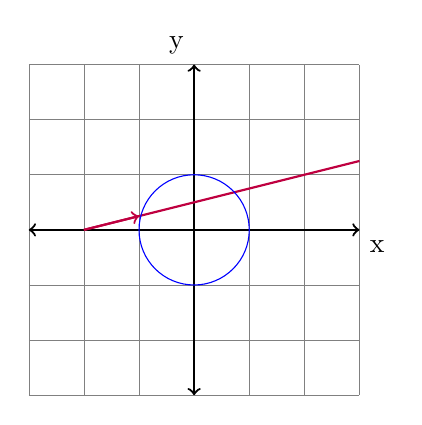
\begin{tikzpicture}[scale=0.7]
        \drawgridaxes
        \draw[purple, thick, ->] (-2,0) -- (-1,0.25);
        \draw[purple, thick] (-2,0) -- (3,1.25);
        \draw[blue] (0,0) circle (1cm);
        \end{tikzpicture}
	}
	
		\frame {
		\begin{equation*} (\vec{s} + t * \vec{d})^2 = r^2
		\end{equation*}
		\begin{equation*} (\vec{s} + t * \vec{d})^2 - r^2 = 0
		\end{equation*}
		\begin{equation*} \vec{s}^2 + t^2 * \vec{d}^2 +2(\vec{s} + t * \vec{d})- r^2 = 0
		\end{equation*}
		\begin{equation*}  t^2 * \vec{d}^2 + t * 2(\vec{s} * \vec{d}) - r^2 + \vec{s}^2 = 0
		\end{equation*}
		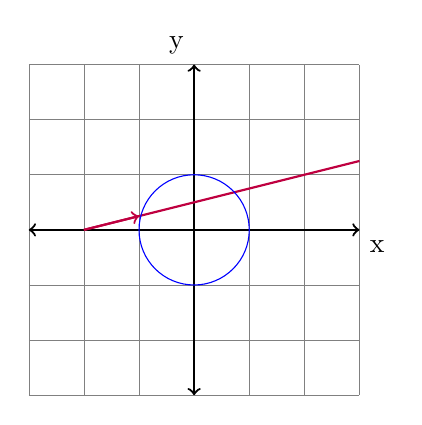
\begin{tikzpicture}[scale=0.7]
        \drawgridaxes
        \draw[purple, thick, ->] (-2,0) -- (-1,0.25);
        \draw[purple, thick] (-2,0) -- (3,1.25);
        \draw[blue] (0,0) circle (1cm);
        \end{tikzpicture}
	}

\end{document}
